%!TEX root = paper.tex

\section{Stream Analytics on Top of Dataflows}
\label{sec:streaming}


Flink’s DataStream API implements a full stream analytics framework on top of Flink’s runtime, including the mechanisms to manage time (including out-of-order event processing), defining windows, and maintaining and updating user-defined state. The streaming API is based on the notion of a DataStream, a (possibly unbounded) immutable collection of elements of a given type. Since Flink’s runtime already supports pipelined data transfers, continuous stateful operators, and a fault tolerance mechanism for consistent state updates, overlaying a stream processor on top of it, essentially boils down to implementing a windowing system and a state interface. As noted, these are invisible to the runtime, which sees windows as just an implementation of stateful operators. 

\subsection{The Notion of Time}
\label{sec:streaming-time}
Flink distinguishes between two notions of time: i) event time, that  stands for the time that an event was generated at its origin (e.g., the time that a sensor or a mobile device generated a signal) and ii) processing time, that is the wall-clock time of the machine that is processing the data.

In distributed systems there is an arbitrary skew between event-time and processing-time \cite{akidau2015dataflow}. This may mean arbitrary delays for getting an answer based on event-time semantics. To avoid arbitrary delays these systems regularly insert special events called ‘low watermarks’ that mark a global progress measure. In the case of time progress for example, that includes a time attribute ‘t’ indicating that all events lower than ‘t’ have already entered an operator. The watermarks aid the execution engine to process events in the correct event order and serialize operations (such as window computations) via a unified measure of progress.

Watermarks originate at the sources of a topology, where we can determine the time inherent in future elements. The watermarks propagate from the sources throughout the other operators of the data flow. Operators decide how they react to watermarks. Simple operations such as map/filter just forward the watermarks they receive, while more complex operators that do calculation based on the watermarks (e.g., event time windows) first compute results triggered by a watermark and then forward it. If an operation has more than one input, the system only forwards the minimum of the incoming watermarks to the operator, ensuring correct results. 

Flink programs that are based on processing time, rely on the machine clocks, and hence a less reliable notion of time, but exhibit lower latency. Programs that are based on event time provide the most reliable semantics, but may exhibit latency due to event time-processing time lag. Flink includes a third notion of time as a special case of event time called ingestion time, which is the time that events enter Flink. This provides  lower processing latency than event time, and more accurate results compared to processing time.


\subsection{Stream Discretization}
Many incremental computations over unbounded streams are often evaluated over finite logical views, called windows. Apache Flink creates windows via a highly flexible discretization process which is composed out of three core functions: a window assigner and optionally a trigger and an evictor. All three functions can be selected among a pool of common predefined implementations (e.g. sliding time window) or explicitly defined by the user (via UDFs).

More specifically, the assigner is responsible for assigning each record to logical windows. For example, this decision can be based on the timestamp of a record when it comes to event-time discretization. Note that in the case of sliding windows, an element can belong to multiple logical windows. An optional trigger defines when the operation associated with the window definition is performed. Finally, an optional evictor determines which records to retain within each window. The discretization operation of Apache Flink is uniquely capable of covering all known window types such as periodic time/count-windows, punctuation, landmark, session and delta windows. Note that windows incorporate out-of-order processing seamlessly as in \cite{li2005semantics, akidau2015dataflow} and, in principle, subsumes these discretization models. For example, below is a window definition of 6 seconds that slides every 2 seconds (Assigner). The window results are computed once the watermark passes the end of the window (Trigger).

\begin{lstlisting}[language=Java]
stream
  .window(SlidingTimeWindows.of(Time.of(6, SECONDS), Time.of(2, SECONDS))
  .trigger(EventTimeTrigger.create())
\end{lstlisting}

A global window creates a single logical group. The following example defines a global window (assigner) that invokes the operation on every 1000 events (trigger) while keeping the last 100 elements (evictor). 

\begin{lstlisting}[language=Java]
stream
  .window(GlobalWindow.create())
  .trigger(Count.of(1000))
  .evict(Count.of(100))
\end{lstlisting}

Note that streams are already partitioned on a key before windowing, so the above is a local operator that does not require coordination between machines. This mechanism can be used to implement a wide variety of windowing functionality \cite{akidau2015dataflow}. 


\subsection{Stateful Stream Processing}
\TODO{Asterios: This is very developer-heavy. We need to show the big picture. Long story short, the side-effect free functional view of the system changes with mutable state that is managed by the system. Why do we need state? What can be state? How is it implemented in Flink. @Paris, please answer these 3 questions in 2-3 paragraphs. The example below could also be missing.}

Simple programs in Flink’s DataStream API look like functional, side effect-free programs consisting of transformations on unbounded immutable collections. However, to cover the need for stateful operations, we incorporate explicit mutable state in the API by providing: $i)$ Operator interfaces or annotations to statically register explicit local variables within the scope of an operation;  $ii)$ an OperatorState abstraction for marking partionable dynamic state and its operations.  Flink’s checkpointing mechanism guarantees that any registered state is durably accessed exactly-once per operation via checkpointing. 

As a simple example consider a map operator that computes a continuous average for a given stocks price. For this we need to keep a state with the current count and total sum for each stock in order to compute the average:


\begin{lstlisting}[language=Scala]
val priceStream: DataStream[(String,Double)] = ...
 
val avgPerStock : DataStream[(String, Double)] = source.keyBy(0).mapWithState(
    (in, state: Option[(Int, Double)]) => {
		val (count, sum) = state.getOrElse((0,0.0))
		val newState = (count + 1, sum + in._2)
		((in._1, newState._2/newState._1), newState)
	}
\end{lstlisting}

\subsection{Fault Tolerance via Asynchronous Snapshots}
\label{sec:fault-tolerance}
The fault tolerance mechanism of Apache Flink for unbounded streams builds on the notion of distributed consistent snapshots/checkpoints to achieve exactly-once-processing guarantees. The possibly unbounded nature of a data stream in the model of the DataStream API makes recomputation upon recovery impractical, as possibly months of computation will need to be replayed considering a long running job. To bound recovery time, Flink takes a snapshot of the state of operators, including the current position of the input streams at regular intervals.

The core challenge lies in taking a consistent snapshot of all parallel operators without halting the execution of the topology. In essence, the snapshot of all operators should refer to the same logical time in the computation. The mechanism used in Flink is called Asynchronous Barrier Snapshotting, or ABS \cite{carbone2015lightweight}. Barriers are control records injected into the input streams that correspond to a logical time, and logically separate the stream to the part whose effects will be included in the current snapshot, and the part that will be snapshotted later.

\begin{figure}[ht]
	\centering  	
  	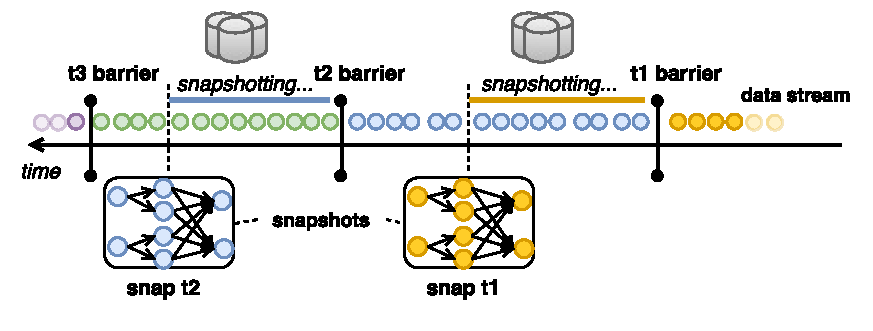
\includegraphics[width=.75\textwidth]{figs/snaps.pdf}
  	\vspace{-6mm}
	\caption{Asynchronous Barrier Snapshotting.}
	\vspace{-2mm}
	\label{fig:snapshots}
\end{figure}

An operator receives barriers from upstream and first performs an alignment phase, making sure that the barriers from all inputs have been received. Then, the operator writes its state (e.g., contents of a sliding window, or custom data structures) to durable storage (the storage backend can be an external system, e.g., HDFS). Once the state has been backed up, the operator forwards the barrier downstream. ABS bears resemblances to the seminal Chandy-Lamport algorithm for asynchronous distributed snapshots \cite{chandy1985distributed}. However, because of the DAG structure of a Flink program, ABS does not need to checkpoint in-flight records but solely rely on the aligning phase to apply all their effects to the operator states. This guarantees that the data that needs to be written to reliable storage is kept to the theoretical minimum (i.e., only the current state of the operators).

Recovery from failures reverts all operator states to their respective states taken from the last successful snapshot, and restarts the input streams starting from the latest barrier. The maximum amount of re-computation needed upon recovery is limited to the amount of input records between two consecutive barriers. Furthermore,  we note that this strategy does not eliminate the possibility for partial recovery, when upstream backup is applied.



\vspace{1mm}
\noindent ABS provides several benefits:\vspace{-3mm}
\begin{itemize}
\item It guarantees exactly-once state updates without ever pausing the computation \vspace{-3mm}
\item It is completely decoupled other forms of control messages, e.g., by events that trigger the computation of windows, thus not restricting the windowing mechanism to multiples of the checkpoint interval. \vspace{-3mm}
\item It is completely decoupled from the mechanism used for reliable storage, allowing state to be backed up to file systems, databases, etc, depending on the larger environment in which Flink is used.
\end{itemize}



